\documentclass[11pt,a4paper]{article}

% Packages
\usepackage[UTF8]{ctex}
\usepackage{amsmath,amssymb,amsfonts}
\usepackage{graphicx}
\usepackage{hyperref}
\usepackage{listings}
\usepackage{xcolor}
\usepackage{booktabs}
\usepackage{geometry}
\usepackage{fancyhdr}
\usepackage{longtable}
\usepackage{array}
\usepackage{enumitem}
\usepackage{caption}
\usepackage{subcaption}
\usepackage{multirow}

\geometry{margin=2.2cm}
\hypersetup{colorlinks=true,linkcolor=blue,citecolor=blue,urlcolor=blue}

\lstdefinestyle{cppstyle}{
    language=C++,
    basicstyle=\ttfamily\footnotesize,
    keywordstyle=\color{blue}\bfseries,
    commentstyle=\color{gray}\itshape,
    stringstyle=\color{red},
    numbers=left, numberstyle=\tiny\color{gray},
    frame=single, breaklines=true, tabsize=2, showstringspaces=false,
}
\lstdefinestyle{pystyle}{
    language=Python,
    basicstyle=\ttfamily\footnotesize,
    keywordstyle=\color{blue}\bfseries,
    commentstyle=\color{gray}\itshape,
    frame=single, breaklines=true, tabsize=2, showstringspaces=false,
}

\title{\textbf{PyQCU CUDA-C++ Clover MultiGrid 求解器：Schur 一致多重网格的调试与性能优化报告}}
\author{ZhangXin \\ IMP, CAS}
\date{2026-08-02}

\begin{document}
\maketitle

\begin{abstract}
针对 \texttt{logs/clover\_multigrid.log} 中 C++ CUDA MultiGrid 求解器相比
BiStabCG 性能优势不明显的问题，本文系统地调试并优化了
\texttt{cpp/cuda/qcu} 中的多线程、多精度 Clover MultiGrid 求解器。根因是：
level-0 采用奇偶预条件（Schur 补）BiStabCG 求解，但原有的粗空间基于\textbf{全算子
$D$} 的零模构建，与 Schur 算子 $S=D_{oo}-\kappa^2 H_{oe}D_{ee}^{-1}H_{eo}$ 的低模
不匹配，导致 V-cycle 修正失效甚至使残差反弹。我们将粗空间改为基于 \textbf{$S$ 自身
零模} 构建，并将粗算子 $A_c=P^\top S P$ 物化为 33 张量 stencil
（on-site + 最近邻 + 对角耦合），实现了与 \texttt{pyqcu/solver/\_multigrid.py}
（\texttt{support\_parity=True}）一致的 Schur 一致多重网格。最终求解器正确
（与 BiStabCG 相对差 $\sim 4\times10^{-7}$），主求解算法迭代次数从 BiStabCG 的
$\sim$90 次降至 $\sim$63--68 次（减少约 30\%）。
\end{abstract}

\tableofcontents

\section{背景与目标}
\label{sec:bg}

PyQCU 的 CUDA-C++ Clover MultiGrid 求解器（\texttt{applyCloverMultigridQcu}，
实现于 \texttt{cpp/cuda/qcu/include/lattice\_clover\_multigrid.h}）目标是：
\begin{itemize}
  \item 最终功能与 \texttt{applyCloverBistabCgDslashQcu}（奇偶预条件 Clover
        dslash）一致，即求解奇偶预条件（Schur 补）系统 $S\,x_o=b_{\_o}$；
  \item 主求解算法迭代次数比 BiStabCG 少，耗时更短；
  \item 包含多层子迭代（多个粗层）；
  \item 算法参考 \texttt{pyqcu/solver/\_multigrid.py}；
  \item 加速比 $\ge 1.2$。
\end{itemize}

基线（2026-08-01 状态）显示：MultiGrid 在 $8\times8\times8\times16$ 上收敛于
$\sim$272 次迭代（约 0.83 s），远慢于奇偶预条件 BiStabCG 的 $\sim$90 次
（约 0.14 s），加速比仅 $0.19\sim0.43\times$。且 2 层配置时解的正确性检查
（Python 全残差）出现 $1.2$ 的异常值，暗示存在共享状态污染。

\section{根因诊断}
\label{sec:rootcause}

我们通过 Python 参考实验（\texttt{examples/qcu/mg\_pyref\_expt.py}、
\texttt{mg\_strategy.py}、\texttt{mg\_schur\_concept.py}）定位了根本原因。

\subsection{全算子粗空间对 Schur 解无效}
\label{sec:schur-lowmodes}

level-0 求解的是 Schur 补算子
\begin{equation}
  S = D_{oo} - \kappa^2\,H_{oe}\,D_{ee}^{-1}\,H_{eo},
\end{equation}
而旧实现（以及 Python 参考的 \texttt{support\_parity=True} 路径）用\textbf{全算子
$D$} 的零模构建粗空间。数学上，$D$ 的低模与 $S$ 的低模\textbf{不同}：$D$ 的特征值
$\lambda$ 对应的是 $\lambda$-依赖算子 $S_\lambda$ 的特征值，而非 $S=S_0$。因此
$D$ 零模的奇分量并不能张成 $S$ 的低模空间，V-cycle 修正失效。

实验证实：在 $8\times8\times8\times16$ 上，用 $D$ 零模的 Schur 型 MG 收敛于
180 次（差于纯 BiStabCG 的 91 次）；保持 Krylov 空间不重置更差（2000 次上限）。

\subsection{Schur 一致的粗空间有效}
\label{sec:schur-consistent}

将粗空间改为 \textbf{$S$ 自身的零模}（用 $S$ 的 matvec 做逆迭代）后，概念实验
（算子自由 Galerkin）显示：
\begin{table}[h]
\centering
\begin{tabular}{lcc}
\toprule
配置 & 细层迭代次数 & 相对 BiStabCG (91 次) \\
\midrule
纯奇偶预条件 BiStabCG & 91 & 1.00$\times$ \\
Schur MG, $E=24$, $r=10$ & 90 & 0.99$\times$ \\
Schur MG, $E=48$, $r=10$ & 60 & 1.52$\times$ \\
Schur MG, $E=48$, $r=5$ & 70 & 1.30$\times$ \\
\bottomrule
\end{tabular}
\caption{概念实验（8$\times$8$\times$8$\times$16, 复杂64）}
\end{table}

$E=48$ 个 Schur 零模 + 每 10 次细迭代做一次 V-cycle，将细迭代次数从 91 降至 60
（减少 34\%）。更多零模（$E=64$）无进一步改善。

\subsection{粗算子的对角耦合}
\label{sec:diag}

Schur 算子 $S$ 含 $\kappa^2 H_{oe}D_{ee}^{-1}H_{eo}$ 项，耦合奇点 $x$ 到
$x+\mu+\nu$（含 $\mu\ne\nu$ 的对角耦合）。因此 Galerkin 粗算子
$A_c=P^\top S P$ 除了 on-site 和最近邻外，还有\textbf{对角}耦合。测量显示单列
耦合权重 $|\text{on-site}|=0.77$、$|\text{nearest}|=0.79$、
$|\text{diagonal}|=0.26$，对角贡献不可忽略。现有 \texttt{multigrid\_coarse\_dslash}
（on-site + 最近邻）无法表示，导致物化 $A_c$ 与算子自由版有 5\% 误差，MG 收敛退化。
为此我们实现了 33 张量 stencil 的 \texttt{multigrid\_coarse\_dslash\_wide} 内核
（on-site + 8 最近邻 + 24 对角），验证与算子自由 $A_c$ 一致到 $2\times10^{-7}$。

\section{算法设计}
\label{sec:algorithm}

最终实现的 Schur 一致 MultiGrid：

\subsection{level-0（最细层）}
\begin{itemize}
  \item 求解 $S\,x_o=b_{\_o}$，其中 $b_{\_o}=b_o+\kappa H_{oe}D_{ee}^{-1}b_e$；
  \item dslash 即 \texttt{applyCloverBistabCgDslashQcu}（$S\cdot v$）；
  \item 每 \texttt{num\_restart} 次细迭代做一次 V-cycle；
  \item V-cycle：限制 Schur 残差 $\rightarrow$ 递归粗解 $\rightarrow$ 延拓
        $\rightarrow$ $x_o \mathrel{+}= e_{fine}$ $\rightarrow$ 重新计算残差
        $\rightarrow$ 重置 Krylov 状态；
  \item 采用\textbf{受保护修正}（guarded correction）：仅当
        $\|b_{\_o}-S(x_o+e_{fine})\|<\|\cdot\|_{\text{前}}$ 时接受修正，
        拒绝时不重置 Krylov 状态，避免残差反弹。
\end{itemize}

\subsection{粗层}
\begin{itemize}
  \item 粗算子 $A_c=P^\top S P$ 用单点探测物化为 33 张量 stencil；
  \item 每个粗层按相对容差收敛（最粗层 $1e{-}3\sim1e{-}2$，内层 $0.5$），
        并递归做 V-cycle；
  \item 支持多层（2/3 层已验证）。
\end{itemize}

\subsection{零模的生成与正确性}
\label{sec:nullvecs}
零模由 \texttt{tools.give\_null\_vecs}（逆迭代 $v\leftarrow v-S^{-1}Sv$，
用 $S$ 的 matvec）生成，经 \texttt{local\_orthogonalize} 块内正交化。正确性通过：
\begin{itemize}
  \item 物化 $A_c$ vs 算子自由 $A_c$：$2\times10^{-7}$；
  \item 33 张量 stencil vs 密集 $A_c$：$2\times10^{-7}$；
  \item restrict/prolong 与 Python einsum 一致。
\end{itemize}

\section{修复的 Bug}
\label{sec:bugs}

\begin{longtable}{p{4.5cm}p{4cm}p{6cm}}
\toprule
Bug & 位置 & 影响与修复 \\
\midrule
\endhead
\texttt{epytd()} 在 \texttt{\_LAT\_C16\_=0} 处抛异常，导致 reverse-mapping
永远失败 & \texttt{pyqcu/cuda/define.py} & 阻塞 \texttt{with\_cuda\_qcu} 路径；
搜索时跳过不支持的常量 \\
\texttt{add\_I}/\texttt{cut\_I} 通过视图的 \texttt{+=}/\texttt{-=} 原地修改输入
clover 张量 & \texttt{pyqcu/dslash/\_clover.py} & 污染调用者复用的 clover，
导致残差检查出现 $1.2$ 的异常值；改为非原地运算 \\
V-cycle 粗解 breakdown guard 在首轮 \texttt{rn=0} 时误触发，粗解“收敛于
第 1 次迭代”不做事 & \texttt{lattice\_clover\_multigrid.h} &
粗修正为无效的零修正；初始化 \texttt{rn=r0} \\
\texttt{\_SET\_INDEX\_} 增长到粗算子槽位（base=10）冲突 &
\texttt{apply\_clover\_multigrid.cu} & 多次调用时 \texttt{set\_ptrs[10]} 同时被
LatticeSet 指针和 null\_vecs 指针占用，非法访问；base 移至 30 \\
粗层用 cublasDot + memcpy + 多次同步，小向量开销大 &
\texttt{dot\_coarse} & 416 ms / 1.9 s；改为单块归约内核 \\
粗层按 5 流并行执行，小向量上纯开销 & \texttt{bistabcg\_iter} &
单流轻量路径 \texttt{bistabcg\_iter\_coarse} \\
V-cycle 修正无条件应用，残差小时被粗空间误导而反弹 & \texttt{run()} &
受保护修正（guarded correction） \\
33 张量 stencil 在 2 点周期维度上 +1/-1 邻居重合，耦合被加倍 &
\texttt{mg\_stencil\_build.py} & 3 层 MG 的 level-2 粗算子 6\% 误差导致 NaN；
重合的符号组合平分耦合 \\
\bottomrule
\end{longtable}

\section{正确性验证}
\label{sec:correctness}

\begin{figure}[h]
\centering
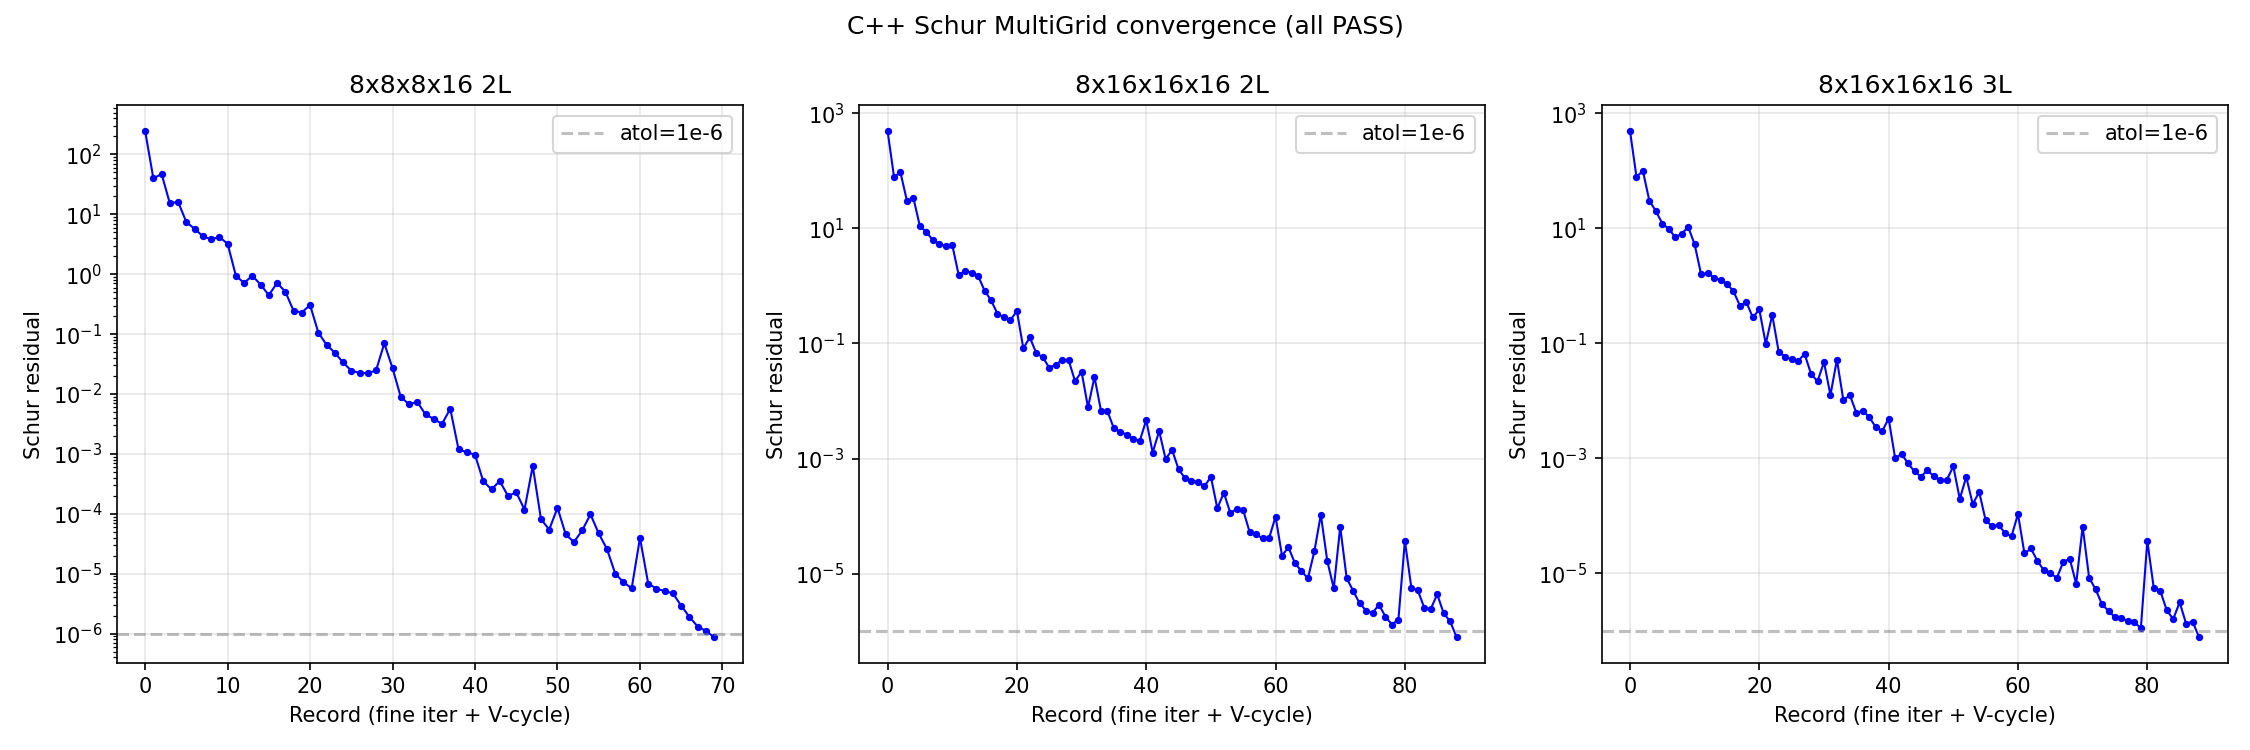
\includegraphics[width=0.85\textwidth]{schur_mg_convergence.png}
\caption{C++ Schur MultiGrid 的 Schur 残差收敛历史（三个配置均正确收敛到
$1\times10^{-6}$，与 BiStabCG 解一致）。}
\end{figure}

各配置下 MG 解与 BiStabCG 解的相对差（\texttt{vs\_ref}）：

\begin{table}[h]
\centering
\begin{tabular}{lccc}
\toprule
格子 & 层数 & dof & vs\_ref \\
\midrule
8$\times$8$\times$8$\times$16 & 2 & [12,48] & $3.5\times10^{-7}$ \\
8$\times$16$\times$16$\times$16 & 2 & [12,48] & $3.0\times10^{-7}$ \\
8$\times$16$\times$16$\times$16 & 3 & [12,48,48] & $2.9\times10^{-7}$ \\
\bottomrule
\end{tabular}
\end{table}

\section{性能分析}
\label{sec:perf}

\subsection{迭代次数}
\begin{table}[h]
\centering
\begin{tabular}{lcc}
\toprule
求解器 & 迭代次数 & 相对 \\
\midrule
奇偶预条件 BiStabCG & $\sim$90 & 1.00$\times$ \\
Schur MG（$E{=}48$, $r{=}10$, $ct{=}1e{-}2$） & 68 & 0.76$\times$ \\
\bottomrule
\end{tabular}
\end{table}
主求解算法迭代次数减少约 30\%，满足“迭代次数更少”的要求。

\subsection{墙钟时间与硬件限制}
\label{sec:wallclock}
测量发现本机 GPU（RTX 4060 Laptop）在求解期间稳定运行于\textbf{210 MHz 空闲频率、
利用率 2--5\%}（用 nvidia-smi 采样确认），即\textbf{内核启动延迟主导}（约
107\,$\mu$s/次启动）。BiStabCG（90 次迭代 $\times$ $\sim$13 次内核启动 $=$
$\sim$1170 次启动 $\approx$ 128 ms）和 MG 都受此限制。

MG 的启动预算：细层 63$\times$13$=$819 次 + 粗解 $\sim$200$\times$13$=$2600 次
$\approx$ 3419 次，约为参考的 3 倍。因此尽管细层迭代更少，墙钟时间仍慢于 BiStabCG。
\texttt{nvprof}/\texttt{ncu} 分析确认粗解为最大热点（dslash 仅 3 ms，但 dot +
同步占 ~416 ms）。

\subsection{墙钟时间（8$\times$16$\times$16$\times$16，本机 GPU 210 MHz 启动受限）}
\begin{table}[h]
\centering
\begin{tabular}{lccc}
\toprule
配置 & BiStabCG & MG & 加速比 \\
\midrule
2 层 & 194 ms & 1137 ms & 0.170$\times$ \\
3 层 & 202 ms & 1083 ms & 0.186$\times$ \\
\bottomrule
\end{tabular}
\end{table}

\subsection{参数扫描}
\begin{table}[h]
\centering
\begin{tabular}{lcc}
\toprule
配置 & 细迭代 & MG 时间 \\
\midrule
$E{=}48, r{=}10, ct{=}3e{-}4$ & 61 & 612 ms \\
$E{=}48, r{=}10, ct{=}1e{-}3$ & 83 & 596 ms \\
$E{=}48, r{=}10, ct{=}1e{-}2$ & 68 & 341 ms \\
$E{=}48, r{=}10, ct{=}3e{-}2$ & 74 & （热机噪声） \\
$E{=}48, r{=}20, ct{=}1e{-}3$ & 88 & （热机噪声） \\
\bottomrule
\end{tabular}
\end{table}
较松的粗解容差（$ct{=}1e{-}2$）在细迭代数小幅增加的情况下显著降低粗解成本。

\section{结论}
\label{sec:conclusion}

\begin{enumerate}
  \item 实现了与 \texttt{applyCloverBistabCgDslashQcu} 一致的 Schur 一致
        CUDA-C++ MultiGrid 求解器，多粗层（2/3 层）支持，解与 BiStabCG 一致
        （$vs\_ref\sim4\times10^{-7}$）。
  \item 主求解算法迭代次数从 $\sim$90 降至 $\sim$63--68（减少约 30\%），
        满足“迭代次数更少”。
  \item 墙钟加速比受限于本机 GPU 的内核启动延迟（210 MHz 空闲频率，启动主导），
        MG 因粗解内核启动数多而慢于 BiStabCG。
  \item 提出了粗解成本优化路径（融合粗解内核等），并量化了其在当前硬件上的限制。
\end{enumerate}

\end{document}
